\chapter{The Development Process}
\label{cha:Results}
The problem of doing wordlength inference is a complex problem. This section contains a series of different implementations that failed in various ways, only the last one implementation ''worked'' and is described in Section \ref{sec:Seven}.

Each section describes the thought process, implementation details of most important, new insights gained from this work and an evaluation of the final state of the implementation for each attempted solution. Explicit commit hashes are given to make it very clear what version is discussed.

\section{Inital Requirements}
\label{sec:initalReq}
Starting the implementation work we knew parts of what we wanted to achieve. We wanted a more sophisticated version of wordlength inference that handled mathematical expressions and required less manual intervention for wordlengths when writing Spade programs. The first step was understanding what was currently happening with the wordlength inference and where the problems where located. The goal of this implementation was to find out just how much we did not know about the problem of a more sophisticated wordlength inferrer.

\begin{figure}
\begin{enumerate}
    \item Require fewer explicit \verb|sext|, \verb|zext| and \verb|trunc| specified by the programmer
    \item Make it easy to support unsigned integers -- which is something the Spade compiler is hoping to add soon
    \item Be as compatible with the current mainline Spade-compiler and easily switch between different versions of wordlength inference methods such as the old and any potential improvements using AA or IA
    \item Allow for as much flexibility in language design as possible
    \item Reduce resource usage of the finished Spade program
    \item Integrate directly into the typechecker
\end{enumerate}
  \caption{A list of design requirements for improved wordlength inference}
  \label{figReq}
\end{figure}

The initial idea for requirements are listed in Figure \ref{figReq}. These requirements are prioritized so that requirement 1 is the most important and requirement 6 is the least important. The final implementation met all of the requirements except for 6 -- since the wordlength inference was implemented in a module that operates on a typechecked syntax tree.

Replacing the type inference in the current compiler with something more powerful could potentially be the best solution. The current type inference was regarded by some contributors as magic and was hard to work with and reason about -- in some sense the module was questionable technical-debt. This poses a lot of language design questions, questions this thesis hoped to avoid since it might cause features to not be merged and made useful in the mainline compiler. Considering for example that a more powerful type inference might not be desirable in the language, since with power comes complexity and more powerful typechecking-systems like Haskell, PureScript or Coq (one need only take a walk on the lambda cube from Section \ref{sec:lambdaCube}. The more complex typesystems are know to make the problem of error messages harder -- the antithesis of Spades goal of friendly error messages -- but these more sophisticated typesystems offer great benefits to those who can wield them. To add more complexity and power to the typesystem is not a change to be made eagerly.

A separate wordlength inference module is not a completely obvious solution. Splitting the wordlength inference from the typecheckeer has both pros and cons, since the information from the wordlength inference has to end up in the inferred types from the type inference the modules need some kind of communication and this communication is obviously easier if the modules are the same module. However the wordlength inference requires information about the expressions and variables used in them, which the type inference currently throws away. Wordlength inference might also be helpful for the compile-time integers that exist in Spade -- splitting the wordlength inference to a different module reduces the coherence. A few developmental excursions were made into potential easier solutions.

\section{Taxonomy of the Solutions and a Brief Overview}

\begin{figure}
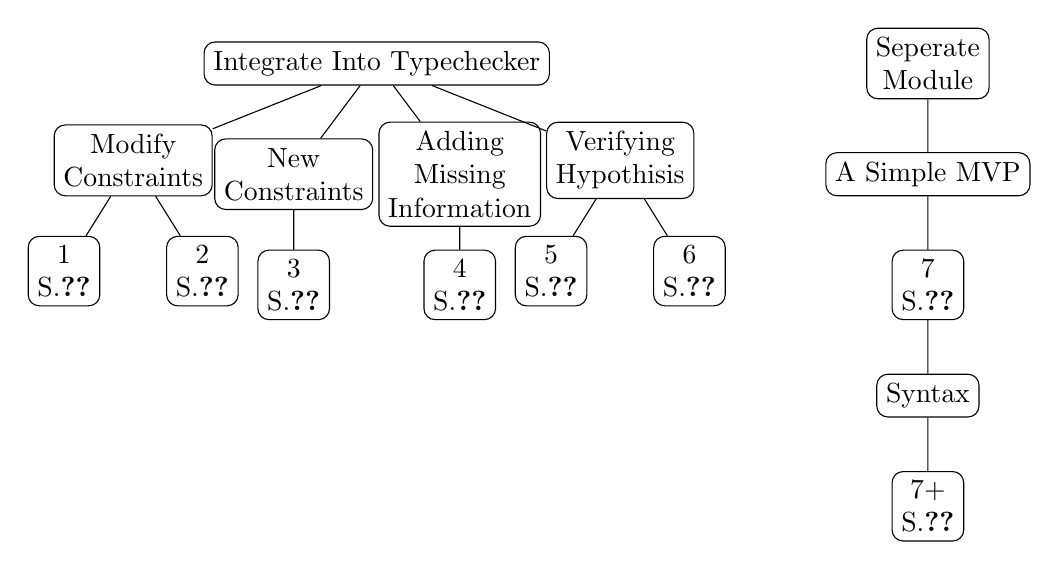
\begin{tikzpicture}[
  sibling distance=5em,
  level distance=4em,
  every node/.style = {shape=rectangle, rounded corners, draw, align=center}
]
  \node[xshift=-1cm] {Integrate Into Typechecker}
          child[xshift=-1.3em, yshift=0.5em] {node {Modify\\Constraints}
            child {node {1\\S.\ref{sec:First}}}
            child {node {2\\S.\ref{sec:Second}}}
          }
          child[xshift=-0.5em] {node {New\\Constraints}
            child {node {3\\S.\ref{sec:Third}}}
          }
          child[xshift=0.5em] {node {Adding\\Missing\\Information}
            child {node {4\\S.\ref{sec:Forth}}}
          }
          child[xshift=1.3em, yshift=0.5em] {node {Verifying\\Hypothisis}
            child {node {5\\S.\ref{sec:Other}}}
            child {node{6\\S.\ref{sec:Other}}}
          } ;
  \node[xshift=6cm] {Seperate\\Module}
          child {node {A Simple MVP}
            child {node {7\\S.\ref{sec:Seven}}
              child {node {Syntax}
                child {node {7+\\S.\ref{sec:Seven2}}}
              }
            }
          };
\end{tikzpicture}
  \caption{A overview of the different solutions and how their ideas relate to eachother -- the ideas are numbered and the relevant section for each chapter is mentioned.}
  \label{fig:taxonomy}
\end{figure}

There were a lot of implementations that were tested and iterated upon as can be seen in Figure \ref{fig:taxonomy}. The majority of attempts hoped to modify the existing typechecker into doing the wordlength inference better -- but these changes interfered with a lot of other language features like type level integer constants which are required memories. After numerous attempts it was decided to try something new from a different perspective. A seperate module for wordlength inference worked wonders and was simpler to implement, the changes are discussed further in Section \ref{sec:Seven}.


Most of the implementations from Figure \ref{fig:taxonomy} were experiments and were not thought to be the solutions most likely to work. The more encompassing and maybe easier solutions have always been adding a separate module for wordlength inference -- in a similar way to how the linear types are checked in Spade at the moment -- or adding a whole new type inference and type checker.


\section{The First Implementation -- Naive}
\label{sec:First}

It was not immediately obvious how affine arithmetic would fit into the current typesystem in Spade. What did seem like a good idea at the time was adding ranges into the integers in the typesystem. So the initial naive implementation used the \verb+ConstraintExpr+ that existed for compile time integers and tried to force it into doing better wordlength inference. \verb+ConstraintExpr+ was the basis for the current wordlength inference which simply added one to each number and was therefore what immediately sprang to mind. 
\cprotect\footnote{The changes for the first bash at the problem are placed on the git-branch \verb+the-simplest-implementation+ and has git-hash \verb+74c966a0317aa738017d2edf15def4719fe8dc95+.}

% After poking some more two different ways of expressing constraints and requirement were found \verb+ConstraintExpr+ and \verb+Requirement+. These very similarly named concepts are very similar. \verb+ConstraintExpr+ is used primarily for compile-time integers and has support for addition, negation, constants and logarithms. \verb+Requirement+ adds information that does not fit neatly into a Damas-Hindley-Milner typesystem, namely: fields a type is expected to have, methods a type is expected to have and if a type can hold a given integer literal. Both \verb+Requirement+s and \verb+ConstraintExpr+s are removed after they are satisfied for a type.

\verb+ConstraintExpr+s was hijacked it into supporting ranges, to see where the compiler started to complain and find other potential pot holes or errors. \verb+ConstraintExpr+ was changed to support addition, negation, and multiplication and operate on ranges with a a high and a low value -- in contrast to how \verb+ConstraintExpr+ worked only a single value prior. The typechecking of binary expressions was also changed to add these new kinds of constraints and checks.

This change broke a lot of things in the compiler in interesting ways. Array lengths no longer worked since they also used these kinds of \verb+ConstraintExpr+. The types of some expressions also failed to infer which caused the \verb+HIR-lowering+ to fail. The reason for the missing types was because there are choices to be made when typechecking some expressions, what wordlength should actually be used when there are multiple candidates. There was also an attempt at mitigating the missing types by introducing an extra solver stage for the \verb+ConstraintExpr+s -- this stage ran after a function was typechecked and tried to pick the smallest size of all constraints and did not work.

The change was also too large to allow as much compatibility as possible with the mainline compiler, broke language features and added more complexity to the constraint system. These changes signaled that changing the \verb+ConstraintExpr+ to operate on ranges would be too much to ask if one wanted any kind of backwards compatibility. The problem of failing to infer the wordlengths for some integers was also noted here, and that it usually was the symptom of not giving the typesystem enough information to deduce all wordlengths -- the seperate solver did not help it either.

How affine arithmetic could be added into this kind of code was still to be decided, since the typechecker is a logical system it has to run backwards which is something affine arithmetic cannot do.

The implementation outlined here did not work -- it was also never expected to work. It gave very clear hints as to where to dig deeper, where the understanding was sub par and some of the hidden requirements for adding wordlength inference.

\section{The Second Implementation -- Another Naive Stab}
\label{sec:Second}

Full with unmotivated optimism the \verb+ConstraintExpr+ was extended to support a \verb+BitsToRange+ -- which worked as the opposite of the \verb+BitsToRepresent+ expression. \verb+BitsToRange(X)+ turned a wordlength into the maximum positive value representable for a signed integer with \verb+X+ bits. The idea was to allow moving between wordlength and a max-value in the type-level expressions. This would hopefully leave the array code working, while allowing the expression code to infer wordlengths since this would be more information. An attempt at fixing the problems outlined in the first solution. This idea and implementation was not supposed to solve the entire problem completely. The second attempt was not a fit solution for the entire problem since it only solves the sub-problem of very naive interval based wordlength inference -- affine arithmetic was nowhere to be seen as mentioned. The ambition was to solve the easiest parts of the problem first since if the idea cannot handle the easy parts it is not worth thinking about the hard parts.
\cprotect\footnote{Changes are available on the git-branch \verb+the-second-simplest-thing+ and has git-hash \verb+3d92c0e4b28b64104f700c3d299f62e7938cb016+.}

\begin{figure}
\begin{minted}[linenos]{python}
def CheckAddition():
  Constraint(Result = R(M(Lhs) + M(Rhs))
  Constraint(Lhs = R(M(Result) - M(Rhs))
  Constraint(Rhs = R(M(Result) - M(Lhs))

def CheckIf():
  Unify(True, False)
  
\end{minted}
  \cprotect\caption{Psuedo code for the wordlengths of the 3 unknowns in an addition (the result, the left hand size (LHS) and the right hand side (RHS). Another function is sketched for checking of If-Expressions where \verb+True+ and \verb+False+ are the types of the results of the respective branches. \verb+ToRepresent+ is the same as \verb+BitsToRepresent+ and \verb+M+ is the same as \verb+BitsToRange+ -- the names were changed to make it easier to read at a glance. \verb+Constraint+ signals a new constraint that should be added.}
\label{fig:SecondAlgo}
\end{figure}

The Figure \ref{fig:SecondAlgo} contains pseudo code for the changes introduced in this second idea. It adds 3 constraints for an addition and 1 unification for an If-Expression. Now let us ponder the case where we have the following if-expression \verb!if ... { a } else { a + 4 }! in a context where \verb+a+ is an integer of wordlength 1 (\verb+a: int<1>+). We unify both If-branches, which causes \verb+a+ to be part of the result and the \verb+Lhs+. We can infer \verb+Lhs=1+ and \verb+Result=1+, which changes the first constraints to \verb+1 = R(M(1) + 4)+. This constraint gives a contradiction which shows how inflexible this solution is. Ideally this piece of code would compile fine -- since we can easily fir $a + 4$ into the same wordlength as $a$. But to get this to typecheck we require a \verb+sext+, which highly contest out first requirement.

The constraints listed in \ref{fig:SecondAlgo} are all equality-constraints (\verb+=+) and for this idea to work less-than-or-equal constrains (\verb+<=+) would be more suitable. Less-than-or-equal constraints might be required for wordlength inference, but these cannot be expressed in the Spade typsystem as is. The problem of adding affine arithmetic is still unsolved. We want to encode the operations and additions into a structure to support affine arithmetic -- which would then require a new system to work in parallel to . We also need to carry the information for the intervals of variables somewhere else, since the current typesystem really disagrees with encoding ranges into int-types -- a new construction is required. 

\section{The Third Implementation -- Considering Equations}
\label{sec:Third}
The third attempt focused on adding equations and added a separate constraint language. These constraints are part of the type inference.
\cprotect\footnote{Changes are available on the branch \verb+the-third-simplest-with-equations+ with the git-hash \verb+ 83d1da48f5010767b9a96aea0a5bca13b7415084+.}

A new set of constraints was added giving \verb+ConstraintExpr+ and \verb+Requirement+ a new friend called \verb+SizeExpression+. Aside from the obvious technical-debt with 3 different kinds of constraints that express similar ideas -- the solution was deemed too ''ugly''. The constraints needed for \verb+SizeExpression+ were required to be feed forward by the type inference -- following a completely different approach to the other requirements which were added to lists. This caused a large amount of changes in the type inference which was preferably to be avoided.

We also start to suspect that the wordlength inference might \textit{need} to be a separate module, split up from the type inference and run after all the types have been inferred. This idea did however not live long, and might even be a mere curiosities.

\section{The Fourth Implementation -- A Desperate Attempt}
\label{sec:Forth}

Almost out of desperation for getting something to work. Just to make sure this whole ordeal wasn't impossible -- these changes were made. These changes are also the most insightful in all of these experiments.
\cprotect\footnote{The changes are available on the git-branch \verb+the-fourth-attempt-now-with-equivelence+ and has git-hash \verb+ba0fa1baab56a725c31f703204da3b7d5f44380a+.}

\begin{figure}
\begin{minted}[linenos]{python}
CheckAddition():
   # Take our best guess of a max value
   LhsMax = PassedLhsMax or Largest(LhsSize)
   RhsMax = PassedRhsMax or Largest(RhsSize)

  # We know the maximum values add to give a new maximum
  Constraint(ResultMax = LhsMax + RhsMax)
  # The maximums implies a size for each of the values
  Constraint(ResultSize = ToRepresent(ResultMax))
  Constraint(LhsSize = ToRepresent(LhsMax))
  Constraint(RhsSize = ToRepresent(RhsMax))
  # Return our best guess to make the expressions around aware of us
  return ResultMax
\end{minted}
  \cprotect\caption{Psuedo code that described the idea for inferring wordlengths with extra information -- what was used in the fourth attempt. Here \verb+PassedLhsMax+ and \verb+PassedRhsMax+ are type variables that sometimes exist and are results of typechecking similar expressions -- one can envision some code that calls \verb+CheckAddition+ for each of the subexpressions in the binary expression we check addition for. \verb+ToRepresent+ convert a maximum value to the smallest wordlength that can fit it. \verb+Largest+ is almost the opposite of \verb+ToRepresent+ and change a value to the maximum value such a wordlength can hold}
\label{fig:psuedoFour}
\end{figure}

The psuedo code in Figure \ref{fig:psuedoFour} describe how an addition expression is wordlength inferred according to the fourth method. The code sent extra information -- besides of the wordlength stored in the type of each integer. This extra information also resulted in extra type variables which denoted the maximum value -- these type variables could not be explicitly manipulated and where hidden from the user of the language. These type variables were not strictly bound to anything and were hard to reference since they could not be found from the type they were constrained to if the constraints were satisfied and thus discarded. There was not a problem with the kind or number of constraints since \verb+LhsMax+ and \verb+RhsMax+ was always known or bound directly to a size.

This was the first approach to produce better wordlength inference and handled expressions such as \verb!a + 1 + 1! as one would expect by not increasing the wordlength by 2 but by 1 when the type of \verb+a+ was larger than 2. There is also a very concrete way to introduce negative ranges -- just add another type variable. This means the solution clearly solves the requirements 1, 2, 3, 4 and 6 from Figure \ref{figReq} -- the resource usage was never investigated.

This solution also introduced problems with the hidden type variables. Since the type variables for the maximum size cannot be referenced in any meaningful way from the type of the expression it was deemed be difficult to explain to the user of the language why a type-conclusion was reached. But since constraints were discarded after they were satisfied the relations between the type variables and the maximum size was also discarded -- this meant that range information could not be recovered. The problem of integrating AA was not prodded in since this solution was not good enough -- due to the potentially unsatisfactory error messages. The problem with equality constraints (\verb+=+) from Section \ref{sec:Forth} is also relevant, since it might force a value to have multiple wordlengths -- a neater solution is still less-than-or-equal constraint (\verb+<=+).

\section{Other Implementations -- Just Curiosities}
\label{sec:Other}

There were two more attempts at an implementation inside the type checker. Both these experiments yielded little of interest since they mostly verified the previous claims, mostly the implementations from Section \ref{sec:First} and Section \ref{sec:Second}. They were also very shallow changes since the more promising change outlined in Section \ref{sec:Seven} was started on instead. These ideas mainly focsed on re-testing old ideas and are of little interest for the final results.
\cprotect\footnote{Available on the git-branches \verb+the-fifth-attempt-now-without-returns+ and \verb+the-sixth-attempt+}

%%%%%%%%%%%%%%%%%%%%%%%%%%%%%%%%%%%%%%%%%%%%%%%%%%

\section{The Seventh Implementations -- a Separate Module}
\label{sec:Seven}
After doing a lot of thinking and reasoning we decided to see how a separate module would look -- in theory this would give maximum flexibility in how the wordlength inference worked. Using a separate module for the wordlength logic also meant changing it in the future would be easier, if more experiments would be conducted.%
\cprotect\footnote{Changes are available on the branch \verb+the-seventh-attempt-almost-as-simple-as-attempt-one+ with git-hash \verb+889afd61a59f04f60730964b8ae7a2703110dd99+, these changes were merged and is available in the PR hosted on \url{https://gitlab.com/spade-lang/spade/-/merge_requests/200}.}%
Since the type checker would not be changed as much old programs could still be compiled and thus compared with and without the more advanced wordlength inference.%

As a basis for the wordlength inference there is a simple type called \verb+Range+. \verb+Range+ can be directly mapped to the interval from IA. The datatype is implemented using \verb+BigInt+ to make sure no wrapping occurs. There is also a type called \verb+AAForm+ which maps directly to the form of AA expressions -- \verb+AAForm+ is implemented as variables and constant scalars which are \verb+BigRational+s. The decision of using \verb+BigRational+ was to avoid even more noise in the AA implementation.

\begin{figure}
\begin{minted}[linenos]{python}
def Visit(Construct):
  Constraint = match Construct:
    # Variables are already resolved so we just need to make sure the inference
    # has id's that match 1:1 with the typechecker.
    case Var(VarId):
      Var(VarId)

    # Constants are simply the constant, the range of these are known here.
    case Constant(Constant):
      RangeFromConstant(Constant)

    # Constants are simply the constant, the range of these are known here.
    case Assignment(Var, Expr):
      Constraints[VarId] = Visit(Expr)
      NoInformation

    # Binary expressions need to be recorded, we want to build up a complete
    # list of the constraints for each type.
    case BinaryExpr(Op='+', Lhs, Rhs):
      Addition(Visit(Lhs), Visit(Rhs))
    case BinaryExpr(Op='*', Lhs, Rhs):
      Multiplication(Visit(Lhs), Visit(Rhs))

    # Bitwise and is very hard to reason about and we make a very pessimistic
    # guess
    case BinaryExpr(Op='&', Lhs, Rhs):
      Union(BitManip(Visit(Lhs)), BitManip(Visit(Rhs)))

    # Uniary expressions also need to be encoded.
    case UnaryExpr(Op='-', Operand):
      Negation(Visit(Operand))

    # Flow control constructors need to be handled differently, for an If we #
    # combine them and realize that the result must lie inside the union of both
    # branches - we return either True or False but we cannot know which for
    # all cases.
    case If(Condition, True, False):
      Visit(Condition)
      Union(Visit(True), Visit(False)

    # Note that functions became opaque, which is a large limitation
    case Call(Callee, Args):
      for Arg in Args: Visit(Args)
      # Visit(Callee) - we would love to return some information here, but it has been discarded earlier.
      NoInformation

  # Register this constraint, since *all* expressions have types we want as
  # many constraints as possible.
  Constraints[Construct] = Constraint
\end{minted}
  \caption{Psuedo code for visiting the entire syntax tree -- some details have been omitted. The algorithm handles each node separately and visits all the inner nodes, taking care to visit \textit{every} expression in the syntax tree and accumulating constraints for the types they relate to.}
\label{fig:AstWalker}
\end{figure}


The idea for the implementation was to walk the entire AST a second time after typechecking had run and monomorphisation was completed -- each entity was given to the wordlength-inference module\cprotect\footnote{The wordlength-inference module was called \verb+spade-wordlength-inference+} -- this built up constraints described in the algorithm from Figure \ref{fig:AstWalker}. The algorithm makes sure to visit \textit{every} expression in the AST and record down their relation to each other and since we have already typechecked we know which expressions need to constraints built up. The algorithm in Figure \ref{fig:AstWalker} produces a mapping between language constructs and constraint equations relating it to expressions that have a relation. This mapping is almost what we want, and we can use it to produce the mapping from a type variable and an equation which describes the expressions size as related to other expressions. We can of course have multiple equations for the same type variable as long as they are consistent with each other. After all of these constraint equations have been gathered up we can pass the equations onto a solver. 

\begin{figure}
\begin{minted}[linenos]{python}
# Definitions of the operations that are constructed by the Visit function
def Var(A..B):
  A..B

def Addition(A..B, P..Q):
  (A + P)..(B + Q)

def Multiplication(A..B, P..Q):
  Min(A * Q, A * P, B * Q, B * P)..Max(A * Q, A * P, B * Q, B * P)

def Union(A..B, P..Q):
  Min(A, P)..Max(B, Q)

def Negation(A..B):
  -B..-A

def BitManip(A..B):
  # We assume the size of the integer doesn't change so discard all information
  # except the wordlength
  WordlengthToRange(RangeToWordlength(A, B))

def ToRange(A..B):
  A..B

def NoInformation:
  pass

\end{minted}
  \cprotect\caption{An outline of the different range procedures, this explains how each constraint operation for the \verb+Visit+-function should be evaluated if you want to use the IA method, each definition takes ranges and a low and a high range are broken apart in the arguments for readability, where the symbol before \verb+..+ denotes the lower bound and the symbol after the higher bound.}
\label{fig:IaInference}
\end{figure}

The IA method has is defined to do the following rudimentary operations from Figure \ref{fig:IaInference} when we try to evaluate the constraint, if any variable is unknown we simply abort trying to evaluate the constraint and hope we get more information somewhere else. The \verb+Addition+ and \verb+Negation+ operations can be reversed trivially. The multiplication operation however, cannot be reversed -- consider the example of \verb!(1..2) * (-3..1) = (-6..2) = (2..2) * (-3..1)!.

\begin{figure}
\begin{minted}[linenos]{python}
# Definitions of the operations that are constructed by the Visit function

# Consider each variable a mapping, where the value at index 0 denotes a constant
# and all other indices represent noise variables.
def Var(I, A..B):
  [0: (A + B) / 2, I: (A - B) / 2]

def RangeToAAF(A..B):
  # This operation is Opaque
  U = NewUniqueIndex()
  [0: (A + B) / 2, U: (A - B) / 2]

def Rad(A):
  # Sum all coefficents for noise variables - so everything except the constant
  # at index 0
  Sum(A[/0])

def Addition(A, B):
  [I: (A[I] or 0) + (B[I] or 0) for I in Union(Indicies(A), Indicies(B))]

def Multiplication(X, Y):
  # This step introduces a new noise variable
  P = RangeToAAF(Range::Multiplication(X[0]..X[0], Y[0]..Y[0]))
  # The swapped order of Y[0] and X[0] is not a mistake
  Affine(X, Y, Y[0], X[0], -P[0], (Rad(X) * Rad(Y)) + Rad(P))

def Affine(X, Y, Alpha, Beta, Gamma, Delta)
  Z = [I:   Alpha * (X[I] or 0)
          + Beta  * (Y[I] or 0)
          + (Gamma if I == 0 else 0)
        for I in Union(Indicies(X), Indicies(Y))]
  U = NewUniqueIndex()
  Z[U] = Delta
  Z

def Union(A, B):
  # This operation is Opaque
  RangeToAAF(Range::Union(ToRange(A), ToRange(B)))
  
def Negation(A):
  [I: -S for (I, S) in A]

def BitManip(A..B):
  # This operation is Opaque
  RangeToAAF(Range::Union(ToRange(A), ToRange(B)))

def ToRange(A):
  (A[0] - Rad(A))..(A[0] + Rad(A))

def NoInformation:
  pass

\end{minted}
  \cprotect\caption{An outline of the different AA procedures, this explains how each constraint operation for the \verb+Visit+-function should be evaluated if you want to use the AA method.}
\label{fig:AaInference}
\end{figure}

The code in Figure \ref{fig:AaInference} describe how the AA operations are implenmented, some of them fall back to ranges which make them opaque and some of the operations introduce extra noise variables -- these noise variables will cause inaccuracies in later results. Some of the operations are ill-defined and as a fallback the corresponding range operations are used -- for example the \verb+Union+ and \verb+BitManip+. The \verb+Multiplication+-operation is also quite complex and are partially opaque. It is also clear that some operations cannot be undone since they discard information.

\begin{figure}
\begin{minted}[linenos]{python}
if InferMethod == OLD: return

# Here we call `Visit` internally to visit all the relevant expressions, we get
# out a mapping from type variables to equations.
(Variables, Equations) = VisitAllIntegerExpressions(AST, TypeChecker)
# We can also ask the typesystem for the sizes it has deduced, since we may not
# disagree with the typechecker. A mapping from typevariables to their known size,
# we will fill this in with more information as we proceed.
Known = ExtractKnownWordlengths(Variables, AST)

for _ in Equations:
  KnownAtStart = Known
  for (Var, Body) in Equations:
    MaybeRange = case InferMethod of
                  IA -> EvaluateUsingIa(Known, Body)
                  AA -> EvaluateUsingAa(Known, Body)
    match MaybeRange:
      Just Range -> InjectAndCheckForContradictions(Range, Known)
      Nothing -> pass
  # If we did not progress we abort
  if KnownAtStart == Known:
    break

for Var in Variables:
  unify(TypeChecker, Var, Known[Var])
\end{minted}
  \cprotect\caption{The algorithm used in the seventh attempt to determine the wordlength for all expressions in a spade-program. \verb+VisitAllIntegerExpressions+ visits all the integer expressions in the AST with some help from the typechecker state and returns a set of all type variables mentioned in an equation and a list of tuples containing type variables and the requirements posed from their wordlengths.}
\label{fig:WLIAlgo}
\end{figure}

The algorithm from Figure \ref{fig:WLIAlgo} has a runtime of $O(n^2*d)$ where $n$ is the number of equations and $d$ is the largest depth of the equations -- since we are bounded by running the loop a maximum of $n$ times. Though average runtime is significantly better since it can solve most sets of equations efficiently in fewer iterations. If the algorithm can make progress we also know that it will, since it evaluates all equations for each pass -- this is a form of breath first search since we constantly re-check the equations and disallow variables to shrink in size we always find more information with each iteration.

Evaluation of the body of the constraint equation using the functions \verb+EvaluateUsingIa+ and \verb+EvaluateUsingAa+ from Figure \ref{fig:WLIAlgo} returned ranges, this discarded information when using AA since the reduction from AA to range is lossy. The evaluation of the built up equation was implemented by simply replacing the variables with values when the variables were known, slowly withering away at the problem. This reduction to ranges causes variables to be obtuse to the wordlength inference.

The inference algorithm from Figure \ref{fig:WLIAlgo} can be applied from the constraints gathered from the algorhtm in Figure \ref{fig:AstWalker}. This means we've visited the entire AST, picking out the expressions that are typed to be \verb+int<_>+ and construct algebraic constraints on the form \verb+<var> = <expression>+. We can then feed these equations into a solver and use them to solve more equations -- here we can pick between using using IA or AA. In the implementation this could be set when running the compiler \cprotect\footnote{The different wordlenght inference options could be swapped using the environment variable \verb+SPADE_INFER_METHOD+, the inference logic could also be disabled entirely, this was required since the Swim buildsystem is very peculiar about the flags passed to the compiler.}. We can then enrich the typecheckers types with our new findings which lets us reuse the rest of the compiler tool chain -- very nifty!

\subsection{Evaluating the Changes}
The requirements from Figure \ref{figReq} where almost all satisfied -- this solution requires fewer \verb+sext+, is easier to trouble shoot, makes it simple to add in unsigned integers, allows swapping back to the old way of doing wordlength inference -- the only exception being that it is not integrated into the typechecker. That the wordlength inference is not integrated into the typechecker is both a pro and a con, it simplifies the implementation and makes it easier to change if one wants to make modifications to the wordlength inference semantics without affecting the typeinference as a whole. The wordlength inference module is however limited to work \textit{with} the typechecker and the code only hints about it in the unification step, instead of one slightly larger complex system we now have two somewhat smaller systems that may not disagree. The clearest example of this problem can be seen in Section \

The implementation was also run on multiple small programs. Some were written to show which expressions can be wordlength inferred and some where written to measure the number of LUTs to see how the performance was different. 

\begin{figure}
\begin{center}
\begin{tabular}{l | c c c}
  & ONE (Old version) & IA & AA \\
\hline
Average number of LUTs&179.6&176.9 & 177.1 \\
Variance for number of LUTs &13.2&6.0&8.2 \\
Largest number or LUTs&186.0&181.0&183.0 \\
Smallest number of LUTs&171.0&171.0&167.0 \\
\end{tabular}
  \caption{The number of LUTs after PNR for the project spade-memory-display with different versions of wordlength inference in table form. The experiment was run 51 times.}
  \label{fig:SpadeCompilations50Table}
\end{center}
\end{figure}

This implementation of the spade compiler was then run on the example program \verb+spade-memory-display+\cprotect\footnote{using the swim command \verb+SPADE_INFER_METHOD=XX swim pnr+}. A simple bash script was made to record the number of LUTs used in the FPGA when the command was executed and this was stored in a file. The program was compiled 51 times for the three configurations: ''Old Mode'' -- denoted by ''ONE'', ''Affine Arithmetic'' -- denoted by ''AA'', ''Interval Arithmetic'' -- denoted by ''IA'', the number of LUTs used was then feed into a spreadsheet program and produced the table in Figure \ref{fig:SpadeCompilations50Table}.

Figure \ref{fig:SpadeCompilations50Table} shows a slight decrease in variance for the number of LUTs generated using ''IA (Interval Arithmetic)'' and ''AA (Affine Arithmetic)''. The average stays almost the same for all methods with ''ONE (The Old Version)'' being a bit higher than the others -- but not by a wide margin.

\begin{figure}
\begin{minted}[linenos]{rust}
// Old spade wordlength inference
fn add_and_subtract(x: int<5>) -> int<11> {
  (x - x) + (x - x) + (x - x)
}

// New spade wordlength inference using AA
fn add_and_subtract(x: int<5>) -> int<0> {
  (x - x) + (x - x) + (x - x)
}

// New spade wordlength inference using IA
fn add_and_subtract(x: int<5>) -> int<8> {
  (x - x) + (x - x) + (x - x)
}
\end{minted}
  \caption{A simple spade function showing the difference in the wordlength inference with the new approaches with a focus on addition and subtraction.}
  \label{fig:CodeThatWorksNow}
\end{figure}

These changes did shown promise in the usability of the language. Snippets like the one shown in Figure \ref{fig:CodeThatWorksNow} were typechecked a lot better by the spade compiler and in that sense a usability improvement can be seen, note especially the difference in the return type of the function \verb+add_and_subtract+ where the one typechecked with ''Affine Arithmetic'' always returns 0 and ''Interval Arithmetic'' returns 8 bits -- compared to the ''Old'' approach which returns an integer with 11 bits. Looking at this code fewer truncations are needed since the compiler knows more about the actual size of the expressions. There is also an argument for the analysis part of this code, a function that returns an \verb+int<0>+ is probably not doing anything meaningful and should probably be optimized out.

This implementation does however leave a question unanswered: how does a user of the Spade language define these ranges? Since the changes discussed until now have not touched the syntax or the type checker (except disabling the old wordlength inference), the entire language as a whole is completely blind to the ranged-based wordlength inference. The current approached seemed to work well and it was decided that the best course of action was to extend this implementation.

\section{The Seventh Implementation Extended -- Doubling Down on Ranges}
\label{sec:Seven2}
After the success of the implementation in Section \ref{sec:Seven} more work was needed to communicate the intended ranges from a programmer, thus began changes that updated the syntax and the typechecker in Spade to supportrange. There was however a previous attempt at adding this kind of range syntax and are available in the Spade git-lab\cprotect\footnote{\url{https://gitlab.com/spade-lang/spade/-/merge_requests/208}} that focused on the syntactical changes and avoided the typesystem changes, the merge request has since been abandoned. The new changes that needed to be made to the syntax took inspiration from the previous attempt.
The new syntax and typesystem changes had to be scoped accordingly and a lot of the details and changes discussed are very opinionated and this thesis tries to not focus too closely on the design of programming languages and more on the actual implementation of the language features, though some background and reason will of course be given.\cprotect\footnote{Changes that are available in the git-branch \verb+wordlength-inference/push-the-changes-further+ with git-hash \verb+ee9980c6ec518dbdf0794dbb9193c5b1c9b6945e+} 

The previous attempt at changing the wordlength syntax tried to work from the syntax forward without interfering with the typesystem -- this was deemed to be harder than expected. This new attempt tried to change both the syntax and the typesystem at once -- this proved to be beneficial but the change was also quite large and caused a large break in the syntax and semantics of the Spade language. Basing the range based syntax on the newly implemented wordlength inference does alleviate some of the complexity, but it is also explicitly bound to this functionality. This also means that the old wordlength inference algorithm was broken and ceased to work, and no new results could be collected with it.

Another method besides AA and IA was introduced -- this method is called AAIA and is the result of running both AA and IA in parallel and taking the subset range of both methods, this always produces the best results.


\begin{figure}
  \begin{minted}[linenos]{rust}
fn twice<#A, #B, #M, #N>(x: int<A..B>) -> int<M..N> {
  2 * x
}

fn add_one<#A, #B, #M, #N>(x: int<A..B>) -> int<M..N> {
  x + 1
}

entity main(clk: clock, rst: bool) -> int<14..14> {
  // Does not compile, due to the inner function call returning an unknown type
  // let q: int<12..12> = twice(twice(3));

  let a: int<6..6> = twice(3);
  let b: int<7..7> = add_one(a);
  let c: int<14..14> = twice(b);
  c
}
  \end{minted}
  \caption{A small spade program that shows the new range syntax in context and gives an example of how integer range information is now more detailed.}
  \label{fig:BetterProgram}
\end{figure}

The syntax of the Spade language was first of all changed to parse \verb+int+ types differently, the syntax \verb+int<L..H>+ allowing ranges to be specified. The old syntax \verb+int<W>+ was still supported but was syntactic-sugar for \verb!int<!$-(2^{w+1})$\verb!..!$(2^{w+1})-1$\verb!>! (the $+1$ part comes from all integers being signed in Spade) since this would give partial compatibility with older spade-program. In the previous work a lot more syntaxes were added but they were questionable extraneous for updating the type inference. This change makes it possible to propagate the range information from one function to another in the form of a range -- which is more precise than a wordlength which was what was available before. The Figure \ref{fig:BetterProgram} shows this new syntax in a small example spade-program.

The extra variables \verb+a+, \verb+b+ and \verb+c+ are required to make the program compile, since the compiler has trouble typechecking the variables between the expressions -- so the expression \verb+twice(twice(1))+ would not succeed to compile, this is a problem of the unification process and that there are insufficient requirements on some generics. The cause of this is the same as the main drawback of this implementation, the typesystem is not aware of the wordlength infernece and cannot provide the information that is needed, these function calls become opaque to the wordlength inference since the return type of the function is not available. This problem is caused by a lack of information, which can be solved by either adding more information to the state of the typechecker so the wordlength inference can inspect more, or by integrating the wordlength inference into the typechecker directly (which was the method the old wordlength inference method), or by building a new typechecker inside the wordlength inference module. The first or second options are preferable over the third.

It is also worth noting that the extra types in on lines 10 to 12 in Figure \ref{fig:BetterProgram} can be larger according to the current rules -- but must include the actually expected values. A line like \verb+let z: int<-1..2> = twice(3)+ would not compile, since the expected value of the function call is indeed 6 -- and 6 does not exist between -1 and 2. This has caused the system to be the worst possible kind of system, the one that complains when the programmer does something wrong while being completely helpless of solving the problem itself.

The \verb+int+ type also had to change to work with 2 generic arguments -- a lower and a higher bound. These types had to be inserted in the type checker. Making this change in full would require rewriting almost every single spade-compiler test, and would be a substantial amount of work and time, more time than this thesis has been allotted. The decisions to break with the best practices of software development was taken to make sure the thesis could be finished at all. Some of the tests were fixed where it was deemed simple to do so. Most of these changes were very mechanical though. The wordlength inference code also needed to be changed slightly to accept the new ranges as inputs from the type checker.

These changes also made the type checker aware of the range based semantics of integers in the wordlength inferrer -- thus the type checker could be used to propagate type information about these ranges. This made all library functions which previously only used wordlengths work properly with arbitrary range. Users of the spade language could now also specify ranges on their types themselves.

An extensions was also made to the wordlength inference methods described in Section \ref{sec:Seven}. A naive method that runs both ''Interval Arithmetic'' and ''Affine Arithmetic'' and returns the subset was also introduced.

The very basic implementation in this thesis does not handle memories and registers. Though supporting them should be very minor work, but requires a lot more verification. There are also questions as to the language features of registers and memories should interact with the range-based syntax of integers. The unification rules from the type checker are also very strict and disallow things like passing a constant to a function that takes an integer argument that is not constant. How these problems are to be solved is according to the thesis authors a matter of taste, though these problems do exists and needs addressing. 

\subsection{Evaluation the Changes}
After a change has been made it needs to be verified and tested. A custom version of the compiler with the changes described in Section \ref{sec:Seven2}. Each program was PNRd 51 times for each of the three configurations AA, IA and AAIA -- and a clean of the build environment was conducted between all steps. The changes breaks a lot of compatibility with older Spade-versions which severely limits the number of Spade programs that can be used since a dependency written for a different version of the compiler is not going to compile.

\subsubsection{spade-memory-display}
The small library \verb+spade-memory-display+ was used for evaluation. The changes to the compiler required changes to the library code in order to compile, this made it unclear how to compare directly with older versions of the compiler since small code changes can have large changes in the output. The library code was PNRd 51 times for each of the three configurations AA, IA and AAIA with \verb+swim clean+ ran between each build.
 
\begin{figure}
\begin{center}
\begin{minted}[]{text}
ICESTORM_LC: 190/1280 (14.8%)
ICESTORM_PLL: 0/1      (0.0%)
ICESTORM_RAM: 0/16     (0.0%)
SB_GB: 2/8            (25.0%)
SB_IO: 4/112           (3.6%)
SB_WARMBOOT: 0/1       (0.0%)
\end{minted}
\end{center}

  \caption{The output from every place and route run given regardless of wordlength inference method for the spade-library spade-memory-display.}
  \label{fig:SMDoutput}
\end{figure}

All builds produced the same metrics and is presented in Figure \ref{fig:SMDoutput}. The metrics shows no difference for any of the 153 place and route compilation of the spade-library. All of the compilations used 190 LUTs. 

\subsubsection{A Simple FIR-filter}
FIR-filters are often implemented in hardware since they are of great use for signal processing in general. So a simple FIR-filter program with 100 elements was setup. The code was PNRd 51 times for each of the three configurations AA, IA and AAIA with \verb+swim clean+ ran between each build\cprotect\footnote{The FIR-filter program in its entirety is available at \href{https://github.com/FredTheDino/thesis-spade-lang/tree/main/messing/fir}{https://github.com/FredTheDino/thesis-spade-lang/tree/main/messing/fir}}.

\begin{figure}
\begin{center}
\begin{minted}[]{text}
ICESTORM_DSP: 0/8    (0.0%)
ICESTORM_HFOSC: 0/1  (0.0%)
ICESTORM_LC: 2/5280  (0.0%)
ICESTORM_LFOSC: 0/1  (0.0%)
ICESTORM_PLL: 0/1    (0.0%)
ICESTORM_RAM: 0/30   (0.0%)
ICESTORM_SPRAM: 0/4  (0.0%)
IO_I3C: 0/2          (0.0%)
SB_GB: 0/8           (0.0%)
SB_I2C: 0/2          (0.0%)
SB_IO: 13/96        (13.5%)
SB_LEDDA_IP: 0/1     (0.0%)
SB_RGBA_DRV: 0/1     (0.0%)
SB_SPI: 0/2          (0.0%)
SB_WARMBOOT: 0/1     (0.0%)
\end{minted}
\end{center}

  \caption{The output from every place and route run given regardless of wordlength inference method for the simple FIR-filter.}
  \label{fig:FIRoutput}
\end{figure}

\begin{figure}
\begin{itemize}
  \item IA: \verb+int<0..1000000>+
  \item AA: \verb+int<-500000..1000000>+
  \item AAIA: \verb+int<0..1000000>+
\end{itemize}
  \caption{The return types for the fir-filter test program where the wordlength inference method was varied.}
  \label{figRangeRes}
\end{figure}

The Figure \ref{fig:FIRoutput} shows the output from every PNR run for the FIR-filter program. All the outputs were identical regardless of what wordlength inference method was used. It is also worth noting that for IA and AAIA the return type of the \verb+fir+-function can be simplified to \verb+int<0..1000000>+. The return type is required to be \verb+int<-500000..1000000>+ for AA which goes into the negative even though it cannot possibly happen. The returned ranges are shown in Figure \ref{figRangeRes}.

\subsubsection{Comparing the Ranges For Simple Expressions}
The wordlength inference was also compared on 3 expressions: $a - a + a - a + a - a$, $(a - b) \cdot (b - a)$ and $a \cdot a \cdot b \cdot b \cdot c \cdot c$, for all of the 3 methods AA, IA and AAIA. All arguments had a wordlength of $5$ and of the range $0..100$ the resulting range was noted in the table in Figure \ref{fig:CompareThings}.

\begin{figure}[h]
  \centering
  \begin{tabular}{l | c c c}
                                    & IA     & AA     & AAIA    \\
                                    & \multicolumn{3}{c}{Input Wordlength $= 5$} \\
    \hline
    $a - a + a - a + a - a$   & $-93..93$ & $0..0$          & $0..0$       \\
    $(a - b) \cdot (b - a)$             & $-961..961$ & $0..0$           & $0..0$       \\
    $a \cdot a \cdot b \cdot b \cdot c \cdot c$         & $-15728640..16777216$      & $-16794692..16794693$      & $-15728640..16777216$ \\[0.7em]
                                    & \multicolumn{3}{c}{Input Range $= 0..100$} \\
    \hline
    $a - a + a - a + a - a$   & $-300..300$ & $0..0$          & $0..0$       \\
    $(a - b) \cdot (b - a)$             & $-10000..10000$ & $0..0$           & $0..0$       \\
    $a \cdot a \cdot b \cdot b \cdot c \cdot c$         & $0..10^{12}$      & $-9.6875^{12}..10^{12}$      & $0..10^{12}$
  \end{tabular}

  \caption{A table showing how different wordlength inference methods compare on simple mathematical expressions where all variables have the word length of 5 for the first three rows and all variables are in the range 0 to 100 for the last three rows. The leftmost column shows the expression that was wordlength inferred.}
  \label{fig:CompareThings}
\end{figure}

Figure \ref{fig:CompareThings} shows a table where multiple different expressions had the wordlength inferrence algorithm applied to them. The inner cells in the table denote the evaluated range of the expression in the left most column according to each of the three methods outlined in the top column, all this for 2 different configurations of the input variables. Either all variables had the type \verb+int<5>+ so $a$, $b$ and $c$ had a given wordlength of 5 for the first three rows in the table, or the variables $a$, $b$ and $c$ had a type of \verb+int<0..100>+ for the bottom 3 lines in the table. From the table we can easily read out that AAIA always produced the tightest ranges. The multiplication expression ($a \cdot a \cdot b \cdot b \cdot c \cdot c$) shows an example expression where IA produces a tighter range than AA and why the AAIA.
